\documentclass[a5j,tombo,10pt,titlepage,pdfusetitle]{ltjsbook}

% LINK
\usepackage{url}
\usepackage{hyperref}
\hypersetup{pdfborder={0 0 0.5}}

% 色の使用
\usepackage{xcolor}
\definecolor{mylinkcolor}{RGB}{3, 112, 145} %{65, 145, 3} % 色定義
\definecolor{linkcol}{RGB}{2, 106, 77} %{65, 145, 3} % 色定義
\hypersetup{
    colorlinks=true,
    citecolor=blue,
    linkcolor=linkcol,
    urlcolor=mylinkcolor % 定義された色
}

% 画像挿入
\usepackage{float}
\usepackage{graphicx}
\usepackage{svg} 

\usepackage{pst-barcode} 

% FONT
\usepackage{fontspec}
% FONT-WEIGHT 調整の指定
% \usepackage[haranoaji,deluxe,nfssonly,jis2004]{luatexja-preset}
\usepackage[haranoaji,deluxe]{luatexja-preset}

% MACRO
\def\ocrb#1{\fontspec{ocrb7} {#1}}
\def\ocrbsmall#1{\fontspec{ocrb7} \fontsize{7}{7}{#1}\selectfont }

\usepackage{framed}

% FONT-SIZE
\def\fs#1#2{\fontsize{#1}{#2}\selectfont }
\def\bf#1{\textbf{#1}}

\title{日本図書コード用バーコード\\ Template with Lua\LaTeX{}\\ \lbrack\ pst-barcode\ \rbrack}
\author{\href{https://github.com/ru-museum?tab=repositories}{ru\_museum}: GitHub)}
\date{\today}

\begin{document}
\thispagestyle{empty}

\maketitle

\setcounter{tocdepth}{2}
\clearpage
\thispagestyle{empty}

\tableofcontents

\newpage
\thispagestyle{empty}

\section{日本図書コード用バーコードの制作}   

\begin{itemize}
  \item 「書籍 JAN コード」には、国際標準 ISBN コード(978-)と日本語書籍で使用されている独自の日本図書コード(192-)とがあります。
  \item 共にエンコード方式は EAN-13 ですが、日本語書籍で使用されている「日本図書コード」としての ISBN バーコードは、国際標準 ISBN バーコードとはその表記法が異なっています(セパレータの有無等)。\vspace{-6mm}\\

\begin{figure}[h]  
\setlength{\unitlength}{0.14in} 
\hspace{10mm}日本図書コード(2段組) \hspace{10mm}国際標準 ISBN コード
\centering                      
\begin{picture}(62,15) 
\put(6,11){\psbarcode{9784003261842}{height=0.45 width=1.28}{ean13}}  
\put(6,10){{\fontspec{ocrb7}9784003261842}}
\put(6,6){\psbarcode{1920197009404}{height=0.45 width=1.28}{ean13}}  
\put(6,5){{\fontspec{ocrb7}1920197009404}}  
 
\put(18,7.7){ 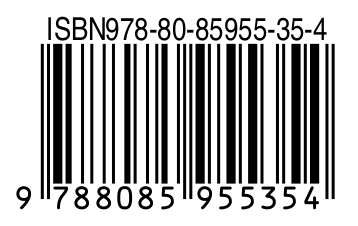
\includegraphics[width=4cm,angle=0]{./images/ean-13-sample.png}} 
\end{picture}  
\end{figure}\vspace{-20mm}\relax  
  \item 現状{}\LaTeX{} での日本図書コード ISBN バーコード作成は用意されていませんので、TexLive 付属の pst-barcode をカスタマイズし利用します。\\  
  {\fs{8}{8}/usr/share/texlive/texmf-dist/tex/latex/pst-barcode(linux: Debian)}
\end{itemize}

\newpage
\section{表記・印刷の規格} 

\begin{itemize}
  \item 書籍 JAN コードの表記・印刷位置は厳密に定められています。\\
{\fs{6}{6}【出典】\href{https://isbn.jpo.or.jp/doc/08.pdf}{ISBNコード/日本図書コード/書籍JANコード利用の手引き 2010年版 ホームページ版}\vspace{-2mm}\\
\hspace{7mm}(日本図書コード管理センター)}

\end{itemize}

\subsection{サイズ} 

{\begin{figure}[H]
\centering
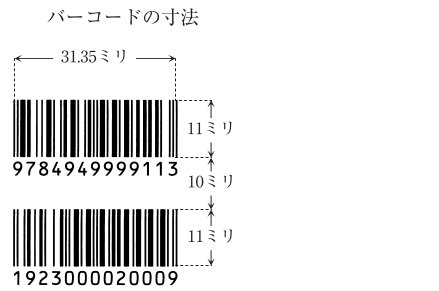
\includegraphics[width=5cm,angle=0]{./images/isbn-layout01.png}
\caption{サイズ規格} 
\end{figure}

\subsection{位置} 

\begin{figure}[H]
\centering
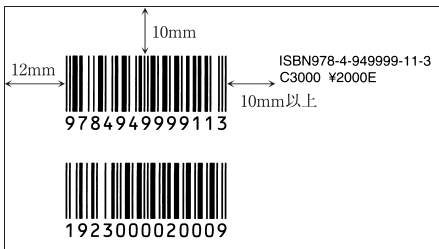
\includegraphics[width=5cm,angle=0]{./images/isbn-layout02.png}
\caption{位置規格(裏表紙左上の場合)} 
\end{figure}


\newpage
\thispagestyle{empty}

\section{作成手順}   

\begin{enumerate}
  \item TexLive 付属の pst-barcode を利用します。\\
  \textbackslash usepackage\{pst-barcode\}
  
  \item 表示は pst-barcode の仕様上バーコード部分のみに適用し、コード番号部分は非表示とし latex で対応しています。\vspace{-2mm}
\begin{verbatim}
{\fontspec{ocrb7}9784003261842}
\end{verbatim}\vspace{-2mm}
{\fs{8}{8}⇒ OCRB フォントについては「0.5 OCRB フォントの使用」を参照して下さい。}

  \item サイズ(高さ、幅)の指定:\vspace{-2mm}
\begin{verbatim}
\psbarcode{9784003261842}{height=0.45 width=1.28}{ean13}
\end{verbatim}\vspace{-2mm}

  \item 表示:\vspace{-8mm}\\
\begin{verbatim}
{\begin{picture}(0,50)(0,20)
\psbarcode{9784003261842}{height=0.45 width=1.28}{ean13}
\end{picture}}\quad\vspace{4.6mm}\\
{\fontspec{ocrb7}9784003261842}
\end{verbatim}\vspace{-12mm}

{\begin{picture}(0,50)(0,20)
\psbarcode{9784003261842}{height=0.45 width=1.28}{ean13}
\end{picture}}\quad\vspace{4.6mm}\\
{\fontspec{ocrb7}9784003261842}\\
\vspace{2mm}
設定値:height=0.45 width=1.28

  \item 各項目の表示位置詳細指定:\\
     ・ 数値を替え正確な位置を設定します。\\
     ・ オフセット値はマイナスを位置することもあります。\\
    \textbackslash begin\{picture\}(160,50)(0,20)\\ 
      \hspace{4mm}( x 方向の長さ, y 方向の長さ )( x のオフセット, y のオフセット)\\ 
    \textbackslash put( x, y )\\ 
    \hspace{4mm}( x のオフセット, y のオフセット)
    
\newpage

  \section*{表示例:}
{\fs{8}{12}
\begin{verbatim}
\begin{picture}(0,0)(-40,120)
\put(-33,76){\psbarcode{9784003261842}{height=0.45 width=1.28}{ean13}}  
\put(-34,66){{\fontspec{ocrb7}9784003261842}}  
\put(-33,13){\psbarcode{1920197009404}{height=0.45 width=1.28}{ean13}}  
\put(-34,3){{\fontspec{ocrb7}1920197009404}}  

\put(92,100){\fontspec{ocrb7}ISBN4-00-326184-4}  
\put(92,78){\fontspec{ocrb7}C0197 \gtfamily{\bfseries¥}940E}  
\put(92,46){\fs{12}{12}{\gtfamily{\mdseries 定価(本体 {\fontspec{Inter-Medium}940}円+税)}}}
\end{picture}
\end{verbatim}
}

\begin{picture}(0,0)(-40,120)

\put(-33,76){\psbarcode{9784003261842}{height=0.45 width=1.28}{ean13}}  
\put(-34,66){{\fontspec{ocrb7}9784003261842}}  
\put(-33,13){\psbarcode{1920197009404}{height=0.45 width=1.28}{ean13}}  
\put(-34,3){{\fontspec{ocrb7}1920197009404}}  

\put(92,100){\fontspec{ocrb7}ISBN4-00-326184-4}  
\put(92,78){\fontspec{ocrb7}C0197 \gtfamily{\bfseries¥}940E}  
\put(92,46){\fs{12}{12}{\gtfamily{\mdseries 定価(本体 {\fontspec{Inter-Medium}940}円+税)}}}
\end{picture}\\  

\end{enumerate}

\newpage
\section{FONT-WEIGHT の調整}

\subsection{luatexja-preset で deluxe を設定} 
\textbackslash usepackage[deluxe]\{luatexja-preset\}

\subsection{フォントの字体指定}\vspace{-10mm} 
\begin{table}[H]
\begin{tabular}{llll}
コマンド & 字体指定 & 表示例 & フォント\\
\hline
   & 標準 & {\fontspec{HaranoAjiMincho-Regular} 戦争と平和 4} & HaranoAjiMincho-Regular\\
  \textbackslash textbf & 太字 & \textbf{\fontspec{HaranoAjiMincho-Regular} 戦争と平和 4} & HaranoAjiMincho-Regular\\
  \textbackslash ltseries & 細字 & \ltseries{\fontspec{HaranoAjiMincho-Bold} 戦争と平和 4} & HaranoAjiMincho-Bold\\
  \textbackslash mdseries & 中字 & \mdseries{\fontspec{NotoSerifJP-Regular} 戦争と平和 4} & NotoSerifJP-Regular\\
  \textbackslash bfseries & 太字 & \bfseries{\fontspec{NotoSerifJP-Bold} 戦争と平和 4} & NotoSerifJP-Bold\\
\end{tabular}
\end{table}

\newpage
\thispagestyle{empty}

\section{OCRB フォントの使用}
\begin{itemize}
  \item \href{https://imagers.co.jp/contents/1537/}{OCRB フォントとは}ISOで規格化された国際規格となっています。
  \item \href{https://ctan.org/pkg/ocr-b-outline}{ocr-b-outline – OCR-B fonts in Type 1 and OpenType}(CTAN)\\
{\fs{9}{9} ※ 従来の .mf フォントは LuaLaTeX では使用出来ませんので OTF を使用します。}
\end{itemize}

\subsection{インストール方法}
\noindent リンク先よりダウンロード・解凍し以下のフォルダに配置します。\\
/usr/share/texlive/texmf-dist/fonts/opentype/public/\textbf{ocr-b-outline}\vspace{-2mm}\\
{\fs{8}{6}
\begin{verbatim}
 ├─ fontforge
 ├─ map
 ├─ opentype
 │  ├── ocrb5.otf
 │  ├── ocrb6.otf
 │  ├── ocrb7.otf
 │  ├── ocrb8.otf
 │  ├── ocrb9.otf
 │  └── ocrb10.otf
 └─ type1
\end{verbatim}\vspace{-5mm}
 ※ 必要があれば \$ fc-cache で更新を行って下さい。}\vspace{-2mm}

\subsection{表示例}\vspace{-2mm}

\noindent\quad\textbackslash ocrb ISBN978-4-06-278761-1\\
{\ocrb\quad ISBN978-4-06-278761-1}\\
\quad\textbackslash ocrbsmall\\
{\ocrbsmall\quad ISBN978-4-06-278761-1}\vspace{-6mm}\\

\noindent \{\textbackslash fontspec\{ocrb7\}ISBN978-4-06-278761-1\}\\
{\fontspec{ocrb7}ISBN978-4-06-278761-1}\\
{\fontspec{ocrb7}ISBN4-00-326184-4 C0197 \textbf{¥}940E}\\
\noindent \{\textbackslash fontspec\{ocrb9\}ISBN4-00-326184-4 C0197 \textbackslash textbf\{¥\}940E\}\\
{\fontspec{ocrb9}ISBN4-00-326184-4 C0197 \textbf{¥}940E}\\

\subsection{「¥」マーク文字について}\vspace{-2mm}
{\fs{9}{9}\begin{itemize}
  \item 「¥」マークは CTAN 版には収録されていませんので、「円記号」を太字化することで補完しています。
  \item 「¥」マークを収録している OCRB.TTF フォントには各社提供のものがあります(MS 社 Windows OS 付属等)が、利用に際しては場合により著作権問題が生じることが有りますので注意して下さい。

\end{itemize}
}

\begin{figure}[H]
\centering
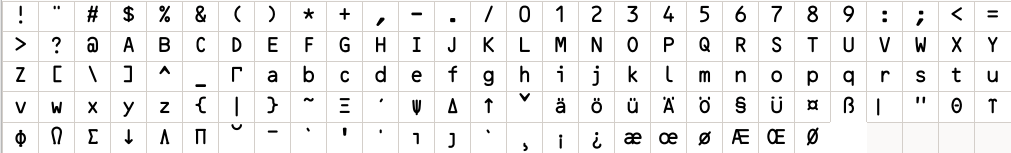
\includegraphics[width=11cm]{./images/ocrb-ttf01.png}
\caption{ocrb7(CTAN)} 
\end{figure}
\begin{figure}[H]
\centering
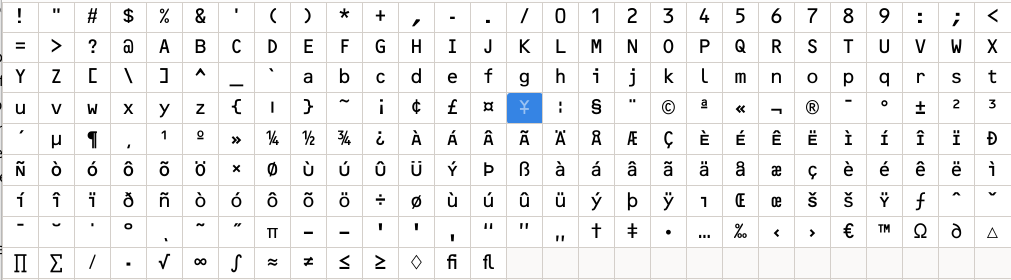
\includegraphics[width=11cm]{./images/ocrb-ttf-ms2.png}
\caption{OCRB.TTF(Microsoft Windows 付属)} 
\end{figure}

\newpage
\thispagestyle{empty}

\section{EXAMPLES}   
\begin{itemize}
  \item 以下掲載のサンプルは、実際の書籍の表示を再現しています。
\end{itemize}

【サンプル書籍】
\begin{table}[H]\fs{8}{8}
\begin{tabular}{llll}
書名 & 著者 & 出版社 & 出版年\\ 
\hline
再発見 日本の哲学 丸山眞男─理念への信 & 遠山敦 & 講談社 & 2010\\ 
戦争と平和 4 & トルストイ/藤沼 貴 訳 & 岩波文庫 & 2006\\ 
夢見る権利 ロシア・アヴァンギャルド再考 & 桑野隆 & 東京大学出版会 & 1996\\ 
岩波講座 言語の科学 9 言語情報処理 & 長尾 真 他著 & 岩波書店 & 1998\\ 
やさしいC & 高橋麻奈 & SoftBank & 2012\\ 
\end{tabular}
\end{table}

\newpage
\thispagestyle{empty}

\begin{picture}(0,0)(0,-10)
\put(0,120){EXAMPLE: 1}   
\end{picture}  

\begin{picture}(0,0)(0,0)

\put(-33,76){\psbarcode{9784003261842}{height=0.45 width=1.28}{ean13}}  
\put(-34,66){{\fontspec{ocrb7}9784003261842}}  
\put(-33,13){\psbarcode{1920197009404}{height=0.45 width=1.28}{ean13}}  
\put(-34,3){{\fontspec{ocrb7}1920197009404}}  

\put(92,100){\fontspec{ocrb7}ISBN4-00-326184-4}  
\put(92,78){\fontspec{ocrb7}C0197 \gtfamily{\bfseries¥}940E}  
\put(92,46){\fs{12}{12}{\gtfamily{\mdseries 定価(本体 {\fontspec{Inter-Medium}940}円+税)}}}
\end{picture}\\  

\vspace{80mm}

\begin{framed}
{\fs{14}{10} \noindent\bf{戦争と平和 4}}\\

{\fs{12}{10}
\noindent トルストイ 作\\ 
 藤沼 貴 訳}\vspace{0mm}\\

\noindent 赤 618-4\\
岩波文庫
\end{framed}

\newpage
\thispagestyle{empty}

\begin{picture}(0,0)(0,-10)
\put(0,120){EXAMPLE: 2}   
\end{picture}  

\begin{picture}(0,0)(0,20)

\put(-33,76){\psbarcode{9784062787611}{height=0.45 width=1.28}{ean13}}  
\put(-34,66){{\fontspec{ocrb7}9784062787611}}  
\put(-33,13){\psbarcode{1920310014001}{height=0.45 width=1.28}{ean13}}  
\put(-34,3){{\fontspec{ocrb7}1920310014001}}  

\put(92,100){\fontspec{Inter-Medium}ISBN978-4-06-278761-1}  
\put(92,86){\fontspec{Inter-Medium}C0310 \gtfamily{\bfseries¥}1400E (0)}  
\put(92,36){\fs{11}{13}{\fontspec{NotoSerifJP-Bold}定価:本体 {\fontspec{GoudyOldStyleSSiSmallCaps}1400}円(税別)}}  
\put(92,16){\fs{11}{12}{\fontspec{NotoSerifJP-Bold}講談社}}  
\end{picture}  

\vspace{100mm}

\begin{framed}
{\fs{14}{10} \noindent\bf{再発見 日本の哲学 丸山眞男─理念への信}}\\

{\fs{12}{10}
\noindent 遠山 敦 著}\vspace{0mm}\\

\noindent 講談社 2010年
\end{framed}


\newpage
\thispagestyle{empty}

\begin{picture}(0,0)(0,-10)
\put(0,120){EXAMPLE: 3}   
\end{picture}  

\begin{picture}(0,0)(0,20)

\put(238,76){\psbarcode{9784130130196}{height=0.45 width=1.28}{ean13}}  
\put(237,66){{\fontspec{ocrb7}9784130130196}}  
\put(238,13){\psbarcode{1911010029877}{height=0.45 width=1.28}{ean13}}  
\put(237,3){{\fontspec{ocrb7}1911010029877}}  

\put(87,100){\fontspec{ocrb7}ISBN4-13-013019-6}  
\put(87,78){\fontspec{ocrb7}C1010 P2987E}  
\put(93,30){\fs{12}{12}\gtfamily{\mdseries 定価{\fontspec{Inter-Medium}2987}円}}  
\put(87.8,16){\fs{12}{12}\gtfamily{\mdseries ({\fontspec{Inter-Medium}本体2900円})}}

%\gtfamily{\mdseries 定価(本体{\fontspec{Inter-Medium}3400}


  
\end{picture}  

\vspace{100mm}

\begin{framed}
{\fs{14}{10} \noindent\bf{夢見る権利 ロシア・アヴァンギャルド再考}}\\
{\fs{12}{10}\noindent 桑野 隆 著}\vspace{0mm}\\
\noindent 東京大学出版会 1996\\
\end{framed}

\newpage
\thispagestyle{empty}

\begin{picture}(0,0)(0,-10)
\put(0,120){EXAMPLE: 4}   
\end{picture}  

\begin{picture}(0,0)(0,20)

\put(238,76){\psbarcode{9784000108591}{height=0.45 width=1.28}{ean13}}  
\put(237,66){{\fontspec{ocrb7}9784000108591}}  
\put(238,13){\psbarcode{1923380034009}{height=0.45 width=1.28}{ean13}}  
\put(237,3){{\fontspec{ocrb7}1923380034009}}  

\put(87,100){\fontspec{ocrb7}ISBN4-00-010859-X}  
\put(87,78){\fontspec{ocrb7}C3380 {\gtfamily{\bfseries¥}}3400E}  
\put(87,30){\fs{12}{12}{\gtfamily{\mdseries 岩波書店}}}  
\put(87,16){\fs{8.2}{12}{\gtfamily{\mdseries 定価(本体{\fontspec{Inter-Medium}3400}円+税)}}}  
\end{picture}  

\vspace{100mm}

\begin{framed}
{\fs{14}{10} \noindent\bf{岩波講座 言語の科学 9 言語情報処理}}\\
{\fs{12}{10}\noindent 長尾 真 他著}\vspace{0mm}\\
\noindent 岩波書店 1998\\
\end{framed}

\newpage
\thispagestyle{empty}

\begin{picture}(0,0)(0,-10)
\put(0,120){EXAMPLE: 5}   
\end{picture}  

\begin{picture}(0,0)(0,20)

\put(238,76){\psbarcode{9784797370980}{height=0.45 width=1.28}{ean13}}  
\put(237,66){{\fontspec{ocrb7}9784797370980}}  
\put(238,13){\psbarcode{1920055025003}{height=0.45 width=1.28}{ean13}}  
\put(237,3){{\fontspec{ocrb7}1920055025003}}  

\put(80,100){\fs{10}{9} \fontspec{Inter-Medium}ISBN4-7973-7098-0}  
\put(80,84){\fs{10}{9} \fontspec{Inter-Medium}C1010 \gtfamily{\bfseries¥}2500E}  
\put(82,32){\fs{12}{12}{\gtfamily{\mdseries 定価 \fbox{本体{\fontspec{Inter-Medium}2,500}円}+税}}}  
\end{picture}  

\vspace{100mm}

\begin{framed} 
{\fs{14}{10} \noindent\bf{やさしいC}}\\
{\fs{12}{10}\noindent 高橋 麻奈 著}\vspace{0mm}\\
\noindent SoftBank 2012\\
\end{framed}

\end{document}

